\section{Verification of TOCL+ Properties}

\hspace{1cm} Figure \ref{sec:verification_approach} presents a comprehensive overview 
of our verification approach for TOCL+ properties. The process begins when a UML 
modeler creates an Application Model and specifies temporal properties using TOCL+. 
Our approach consists of three sequential transformation and verification steps:

First, we transform the Application Model into a Filmstrip Model. This crucial step 
converts dynamic specifications into static ones by representing the system's behavior 
through a sequence of snapshots and operation calls. The Filmstrip Model effectively 
flattens temporal behavior into a structural representation that can be analyzed 
using static verification techniques.

Second, we translate the TOCL+ properties into equivalent OCL expressions interpreted 
over the Filmstrip Model. These OCL expressions navigate through snapshots and 
operation calls, ensuring that the temporal constraints are properly enforced across 
the system's execution. The translation process systematically converts temporal 
operators and event constructs into path expressions over the filmstrip structure.

Third, we verify the resulting OCL expressions using the USE Model Validator 
\cite{USE_Validator}. This static analysis tool examines the Filmstrip Model against 
the translated constraints within a configurable search space defined in a properties 
file. The validator explores possible system states, reporting either SATISFIABLE 
(when a valid system state exists that satisfies all constraints) or UNSATISFIABLE 
(when no valid state can satisfy all constraints simultaneously).

\begin{figure}
    \centering
    \includegraphics[width=1\textwidth]{figures/c2/Verification_approach_1.png}
    \caption{Verification approach.}
    \label{sec:verification_approach}
\end{figure}

In the following subsections, we explain each step in detail using our Software 
System example from Figure \ref{fig:class_diagram_software_system}.


\subsection{Step 1: Transforming the Application Model into a Filmstrip Model}

\hspace{1cm} The first step in our verification approach applies the filmstripping 
technique (described in Section~\ref{subsec:filmstripping}) to transform our Software 
System model into a static representation. Rather than repeating the general 
transformation process, we focus here on the specific application to our example 
and how it enables subsequent verification steps.

For our Software System model from Figure \ref{fig:class_diagram_software_system}, 
the filmstrip transformation preserves the original classes (\texttt{System} and 
\texttt{Application}) and their associations while introducing the filmstrip 
infrastructure. The four operations in our model—\texttt{load(app:~Application)}, 
\texttt{install()}, \texttt{run(app:~Application)}, and 
\texttt{stop(app:~Application)}—are each transformed into concrete 
\texttt{OperationCall} subclasses that capture their specific parameters and context.

The critical aspect of this transformation is how it represents temporal behavior 
through structural relationships. Each snapshot in the resulting filmstrip model 
corresponds to a distinct point in time, with operation calls connecting these 
snapshots to form execution sequences. This structural representation allows us to 
track how object states change over time, which is essential for verifying temporal 
properties.

The transformation of operation contracts is particularly important for our 
verification approach. Consider the pre- and postconditions for the \texttt{load} 
operation shown in Listing~\ref{lst:pre_post_load}. These conditions are transformed 
into invariants in the filmstrip model, as shown in 
Listing~\ref{lst:invariants_load_SystemOpC}. For example, the postcondition 
\texttt{loaded} becomes an invariant that navigates between pre- and post-operation 
states using \texttt{succSystem} and \texttt{predSystem} associations.

The resulting filmstrip model was previously illustrated in Figure 
\ref{fig:filmstrip_model} in Chapter 1, showing how the original application model 
is extended with filmstrip-specific elements. This structural representation of 
system behavior forms the foundation for the next steps in our verification approach, 
allowing us to express and check temporal properties as static constraints over the 
filmstrip model.

\begin{lstlisting}[
    style=toclstyle, 
    caption={Pre and post conditions for load operation.}, 
    label={lst:pre_post_load}
]
context System::load(app: Application)
    pre notLoaded: 
        not self.loadedApps->includes(app) and
        not self.installedApps->includes(app) and
        not self.runningApps->includes(app)
    pre enoughMemory: 
        self.freeMemory >= app.size
    post loaded: 
        self.loadedApps = self.loadedApps@pre->including(app)
    post reduceMemory: 
        self.freeMemory = self.freeMemory@pre - app.size
\end{lstlisting}

\begin{lstlisting}[
    style=toclstyle, 
    caption={Invariants for load\_SystemOpC}, 
    label={lst:invariants_load_SystemOpC}
]
context load_SystemOpC 
inv pre_notLoaded:
    not aSelf.loadedApps->includes(app) and 
    not aSelf.installedApps->includes(app) and 
    not aSelf.runningApps->includes(app)

context load_SystemOpC 
inv pre_enoughMemory:
    aSelf.freeMemory >= app.size

context load_SystemOpC 
inv post_loaded:
    aSelf.succSystem.loadedApps = 
    aSelf.succSystem.predSystem.loadedApps->collectNested( a1:Application | 
        a1.succApplication 
    )->asSet()->including(app.succApplication)

context load_SystemOpC 
inv post_reduceMemory:
    aSelf.succSystem.freeMemory = 
    aSelf.succSystem.predSystem.freeMemory - app.succApplication.size
\end{lstlisting}


\subsection{Step 2: Translating TOCL+ Properties into OCL Expressions}

\hspace{1cm} After transforming the application model into a filmstrip model, the 
second step of our verification approach involves translating TOCL+ temporal 
properties into equivalent OCL constraints. These constraints must be expressed in 
terms of the filmstrip model structure created in Step 1, allowing them to be 
verified using standard OCL tools.

The translation process begins with temporal properties specified in TOCL+ for the 
original Software System model. Each TOCL+ property is systematically transformed 
into an OCL constraint that navigates through the filmstrip structure of snapshots 
and operation calls. This transformation preserves the semantic meaning of the 
original temporal specifications while expressing them through the structural 
elements of the filmstrip model.

Listing \ref{lst:tocl+} shows the original TOCL+ properties specified for our 
Software System model, including safety and liveness properties. As an example of 
the translation process, Listing \ref{lst:ocl_liveness} presents the OCL translation 
for the liveness property, demonstrating how temporal requirements are mapped to 
structural constraints within the filmstrip framework. The translation uses snapshot 
navigation and operation call existence checks to capture the temporal semantics of 
the original property.

\begin{lstlisting}[
    style=toclstyle, 
    caption={OCL translation of liveness property.}, 
    label={lst:ocl_liveness}
]
context System
inv liveness:
    self.loadedApps->notEmpty() implies
    self.loadedApps->forAll(app |
        (let CS:Snapshot = self.snapshotSystem in 
        Set{CS}->closure(s | s.succ())->excluding(null)->exists(s | 
            install_SystemOpC.allInstances()->exists(op | op.succ() = s)
        ))
    )
\end{lstlisting}

The resulting OCL constraints serve as the input for the verification step that 
follows, where they will be evaluated against potential system states to determine 
if the model satisfies the specified temporal properties. While this section has 
provided an overview of the translation approach, the detailed implementation 
of the transformation process from TOCL+ to OCL will be presented in the next section
(Section \ref{sec:translation}).
% The resulting OCL constraints serve as the input for the verification step that 
% follows, where they will be evaluated against potential system states to determine 
% if the model satisfies the specified temporal properties. The detailed implementation 
% of the interpretation process will be presented in Chapter 3.


\subsection{Step 3: Verifying the translated OCL expressions}

\hspace{1cm} The final step in our verification approach employs the USE Model 
Validator \cite{USE_Validator} to verify the OCL constraints generated in Step 2 
against our filmstrip model. This verification process determines whether the 
original TOCL+ properties are satisfied by the application model. The Model Validator 
systematically explores possible system states using a boolean satisfiability (SAT) 
solver, searching for valid instances of the filmstrip model that satisfy all 
constraints or demonstrating that no such instance exists.

Before verification, we configure the search space through a properties file 
(.properties) that establishes bounds for model elements including types, classes, 
and associations. These bounds define the scope within which the Model Validator 
explores possible system configurations. Listing \ref{lst:configuration_file} shows 
one specific configuration used in our Software System example.

\begin{figure}[htbp]
    \begin{minipage}[t]{0.48\textwidth}
    \begin{lstlisting}[basicstyle=\ttfamily\scriptsize, frame=single]
    Integer_min = 0
    Integer_max = 100
    String_max = 10
    Real_min = -2.0
    Real_max = 2.0
    Real_step = 0.5
    
    ### Classes
    # Snapshot
    Snapshot_min = 3
    Snapshot_max = 3
    # Filmstrip
    Filmstrip_min = 2
    Filmstrip_max = 2
    # System
    System_min = 3
    System_max = 3
    # Application
    Application_min = 6
    Application_max = 6
    
    ### Operation Classes
    # load_SystemOpC
    load_SystemOpC_min = 1
    load_SystemOpC_max = 1
    # install_SystemOpC
    install_SystemOpC_min = 1
    install_SystemOpC_max = 1
    \end{lstlisting}
    \end{minipage}
    \hfill
    \begin{minipage}[t]{0.48\textwidth}
    \begin{lstlisting}[basicstyle=\ttfamily\scriptsize, frame=single]
    # run_SystemOpC
    run_SystemOpC_min = 0
    run_SystemOpC_max = 0
    # stop_SystemOpC
    stop_SystemOpC_min = 0
    stop_SystemOpC_max = 0
    
    ### Associations
    # SnapshotSystem
    SnapshotSystem_min = 3
    SnapshotSystem_max = 3
    # SnapshotApplication
    SnapshotApplication_min = 6
    SnapshotApplication_max = 6
    # PredSuccSystem
    PredSuccSystem_min = 2
    PredSuccSystem_max = 2
    # PredSuccApplication
    PredSuccApplication_min = 4
    PredSuccApplication_max = 4
    # SystemApplication
    SystemApplication_min = 6
    SystemApplication_max = 6
    
    ### Additional configurations
    aggregationcyclefreeness = on
    forbiddensharing = on
    \end{lstlisting}
    \end{minipage}
    \caption{Configuration file used for Fig. \ref{fig:object_diagram_liveness}.}
    \label{lst:configuration_file}
\end{figure}

When executed with these parameters, the Model Validator attempts to find a valid 
model instance that satisfies all constraints—including both the filmstrip model 
invariants and our translated temporal properties. If such an instance exists, the 
validator produces an object diagram as evidence; otherwise, it reports that the 
properties cannot be satisfied within the given search bounds.

Figure \ref{fig:object_diagram_liveness} displays an object diagram returned by the 
Model Validator checking against our liveness property. This diagram illustrates a scenario where 
the system first loads and then installs an application—a sequence that satisfies our 
liveness requirement. The diagram shows three snapshots representing the system's 
state at different points in time, connected by two operation calls: \texttt{load} 
followed by \texttt{install}.

\begin{figure}
    \centering
    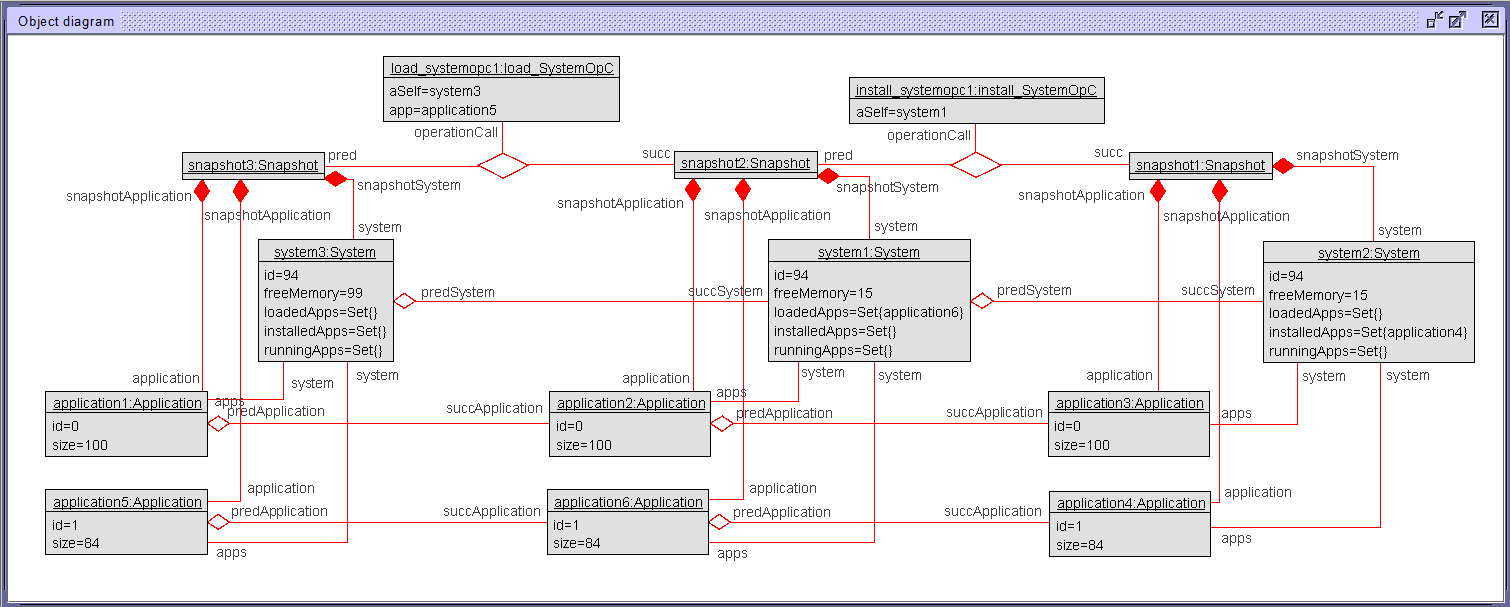
\includegraphics[width=1\textwidth]{figures/c2/ObjectDiagram_Liveness_LoadInstall.png}
    \caption{Object Diagram returned by the Model Validator.}
    \label{fig:object_diagram_liveness}
\end{figure}

You may notice the custom \texttt{id} attribute present in Figure \ref{fig:class_diagram_software_system}
and Figure \ref{fig:object_diagram_liveness}. We manually added this attribute to help 
identify corresponding objects across different snapshots. For example, the scenario 
shows three Application objects with an identical \texttt{id} value of 0, indicating 
they represent the same logical entity at different points in time. This attribute 
is not part of the standard filmstrip model, and we will explain the implementation 
details and necessary constraints for maintaining object identity in section \ref{sec:translation}. 
This validation confirms that our Software System model can satisfy the temporal 
behavior specified by the liveness property.
    